\renewcommand{\CODELOC}{c/ch4/}

\chapter{Nonlinear elliptic PDEs on structured grids}
\label{chap:nonlinear}

\section{Newton's method}

How should nonlinear equations first appear in a code which uses \PETSc?  The answer is that they merely change the functional form of the residual.  For a linear system the residual is this function of the unknowns,
\begin{equation}
\br = \bF(\bu) = \bb - A \bu, \label{eq:nl:linres}
\end{equation}
but we now consider cases in which function $\bF(\cdot)$ is a higher-order polynomial, a transcendental function, or some more general function.  That is, we suppose $\bF : \RR^N \to \RR^N$ is differentiable.  The input $\bx$ and output $\bF(\bx)$ are column vectors,\sidenote{The name change of the unknown $\bu\to\bx$, relative to \eqref{eq:nl:linres}, is because we will now think more geometrically about changes in the location of $\bx$.} so in that sense $\bF$ acts like multiplying by a square matrix $\bx\mapsto A\bx$.  Just as we would reduce the residual to zero in an iterative linear algebra method, for nonlinear $\bF$ we want to solve
\begin{equation}
   \bF(\bx) = 0   \label{eq:nl:equation}
\end{equation}
by iteration.

In this section we follow Isaac Newton in building an iterative method to solve \eqref{eq:nl:equation}.  This method linearizes \eqref{eq:nl:equation} around the most recent iterate and then ``moves'' $\bx$ to the location which solves the linear problem and is, we hope, closer to the solution.  Each iteration therefore solves a linear system; we already have some \PETSc technology for that!  However, choosing the ``smart'' distance to move will require additional choices.  Furthermore, the cost of performing the linearization must be taken into account, and all existing issues regarding the linear solver, including preconditioner choices, as discussed in the last two chapters, remain active.

Of course, nonlinear PDEs do arise in applications.  They come from physical models with nonlinearities, and we will see examples later in this section.  Discretizing nonlinear PDEs leads to systems like \eqref{eq:nl:equation}, and we will give examples of that.  For now, however, we concentrate on solving \eqref{eq:nl:equation}.

First we recall Newton's method.  If we had determined a step $\bs$ from the current iterate $\bx_k$, where both are vectors in $\RR^n$, we would let $\bx_{k+1} = \bx_k + \bs$ be the next iterate.  By definition, because $\bF$ is differentiable,
\begin{equation}
    \bF(\bx_{k+1}) = \bF(\bx_k) + J_\bF(\bx_k) \bs + o(\|\bs\|)  \label{eq:nl:expandF}
\end{equation}
for some square matrix
\begin{equation}
J_\bF(\bx_k) = \begin{bmatrix}
    \frac{\partial F_0}{\partial x_0} & \dots & \frac{\partial F_0}{\partial x_{N-1}} \\
    \vdots & \ddots & \vdots \\
    \frac{\partial F_{N-1}}{\partial x_0} & \dots & \frac{\partial F_{N-1}}{\partial x_{N-1}}  \end{bmatrix},  \label{eq:nl:jacdefn}
\end{equation}
and where $o(\|\bs\|)$ denotes some quantity that goes to zero as the length of the step $\|\bs\|$ goes to zero.  The matrix $J = J_\bF(\bx_k)$ is called the \emph{Jacobian} of $\bF$ at $\bx_k$, though we also refer to the function $\bx \mapsto J_\bF(\bx)$ as the Jacobian.

An iteration of Newton's method approximately solves nonlinear equation \eqref{eq:nl:equation} by truncating \eqref{eq:nl:expandF} and then seeking $\bs$ so that the updated value $\bF(\bx_{k+1})$ is zero.  That is, each Newton step computes $\bs$ by the equation
\begin{equation}
    0 = \bF(\bx_k) + J_\bF(\bx_k) \bs.
\end{equation}
Writing this equation in our previous style ``$A\bu=\bb$'' for linear systems, at each iteration $k$ we solve a linear system and then do a vector addition:
\begin{align}
    J_\bF(\bx_k) \bs &= - \bF(\bx_k)  \label{eq:nl:newtoneq}  \\
    \bx_{k+1} &= \bx_k + \bs  \label{eq:nl:newtonupdate}
\end{align}
This is Newton's method.  It is simple in theory.

Actual practice is not that much more complicated, especially with \PETSc in hand.  Despite the reputation of Newton iteration as fragile or scary, by using a bit of caution in ``moving'' to the new iterate as in \eqref{eq:nl:newtonupdate}, this will work out just fine on many small nonlinear systems \citep{Kelley2003}.  On big nonlinear systems we will need to pay more attention to the details of the linear solve at each step.\sidenote{It is important to emphasize that the nonlinear problem requires all of the tools for linear systems already considered in Chapters \ref{chap:linearsystem} and \ref{chap:structured}, and more.}  In either case, Newton iteration is the core technology for solving nonlinear problems, including nonlinear PDEs.

A small example gives us a start on exploring the details.

\medskip\noindent\hrulefill
\begin{example}  Nonlinear systems can be visualized as the intersections of curves, surfaces, or hypersurfaces, depending on dimension.  For example, given $b > 1$ this pair of nonlinear equations
    $$y = \frac{1}{b} e^{bx}, \qquad x^2+y^2 = 1,$$
form intersecting curves in the plane.  As shown in Figure \ref{fig:expcirclebasic} for the $b=2$ case, the curves intersect twice, once each in the first and second quadrants.

These equations are put in standard form \eqref{eq:nl:equation} by writing
\begin{equation}
\label{eq:nl:expcircleF}
\bF(\bx) = \begin{bmatrix}
           \frac{1}{b} e^{b x_0} - x_1 \\
           x_0^2 + x_1^2 - 1
           \end{bmatrix}
\end{equation}
for $\bx\in \RR^2$ with components $\bx = [x_0 \, x_1]^\top$.  Thus
\begin{equation}
\label{eq:nl:expcircleJac}
J_\bF(\bx) = \begin{bmatrix}
    e^{b x_0} & -1 \\
    2 x_0   & 2 x_1 \end{bmatrix}
\end{equation}
Let $b=2$.  If we start the Newton iteration with $\bx_0 = [1 \, 1]^\top$ then the sequence of iterates from \eqref{eq:nl:newtoneq} and \eqref{eq:nl:newtonupdate} is
    $$\twovect{\bx}{0}{1}{1}, \quad \twovect{\bx}{1}{0.619203}{0.880797}, \quad \twovect{\bx}{2}{0.394157}{0.948623}, \quad \dots$$
as also shown in Figure \ref{fig:expcirclebasic}.

\noindent\hrulefill
%  FROM $ for N in 0 1 2; do ./expcircle -snes_fd -snes_max_it $N; done
\end{example}

\begin{marginfigure}
\includegraphics[width=1.2\textwidth]{expcirclebasic}
\caption{Newton iterates approach a solution of $\bF(\bx)=0$ for $\bF$ in \eqref{eq:nl:expcircleF} and $b=2$.}
\label{fig:expcirclebasic}
\end{marginfigure}


\section{\pSNES and call-backs}

We will do this calculation in \PETSc using a nonlinear-solver object of type \pSNES, an acronym which stands for ``scalable nonlinear equation solver.''  This object has the usual \texttt{Create/SetFromOptions/Destroy} sequence.  A \pSNES object also has a method by which we tell it about the function $\bF$.  This is a ``call-back'' in the sense that we supply a function which the \pSNES can call, inputing argument $\bx$ when it needs $\bF(\bx)$ during the Newton iteration.  In further examples we will also provide the \pSNES with a function which computes the derivative of $\bF$, i.e.~we will provide the Jacobian function $J_{\bF}$, but because this derivative can optionally be approximated by finite differences, our first code can avoid a ``call-back'' for the Jacobian.

Figure \ref{code:expcircle} shows our first \pSNES-using code \texttt{expcircle.c}.  It solves problem \eqref{eq:nl:equation} with $\bF$ from \eqref{eq:nl:expcircleF} and $b=2$.  The \texttt{main()} portion is mostly not surprising, but we summarize the contents anyway:  We start by allocating \pVec \texttt{x}, of fixed dimension 2, which will hold both the initial iterate $\bx_0$ and, once the Newton iteration is ended, the converged estimate of the solution to system \eqref{eq:nl:equation}.  Because both components of $\bx_0$ are $1$ in the above example, it is easy to initialize the \pVec with \texttt{VecSet()}.  Next a duplicate \pVec \texttt{r} is created because we need to supply it to the \pSNES as space for the (nonlinear) residual.  Then the \pSNES is created and configured by a \texttt{SNESCreate()} call which is totally uninteresting.  Next the formula \eqref{eq:nl:expcircleF} is supplied by a call to \texttt{SNESSetFunction()}.  This ``call-back'' sets the third argument of \texttt{SNESSetFunction()} to the name of the C function \texttt{FormFunction()}, which also appears in Figure \ref{code:expcircle}.  Next \texttt{SNESSetFromOptions()} is called so that, in particular, we will have run-time control both on how the Jacobian is calculated and on how the length of the step $\bs$ is actually determined; see below.  Then the system is solved by a call to \texttt{SNESSolve()}, which also supplies the initial iterate, and space for the solution, in \texttt{x}.  Finally the new state of \texttt{x}, presumably the converged solution, is printed at the command line using \texttt{VecView()} with a \texttt{STDOUT} viewer.

\vfill
\cinput{expcircle.c}{\CODELOC}{A first \pSNES-using code.  Solves nonlinear system \eqref{eq:nl:equation} with $\bF$ given in \eqref{eq:nl:expcircleF}.}{//START}{//END}{code:expcircle}

In order to match the calling sequence of \texttt{SNESSetFunction()}, our \texttt{FormFunction()} must have a particular ``signature'' as a C function:
\begin{code}
PetscErrorCode (*f)(SNES,Vec,Vec,void*)
\end{code}
That is, \texttt{FormFunction()} must have the \pSNES, the input $\bx$ (as the first \pVec), the output $\bF(\bx)$ (as the second \pVec), and perhaps additional information. such as parameters, in a ``user context;'' we will return to ``user contexts'' below.

Looking inside \texttt{FormFunction()} in Figure \ref{code:expcircle} we see new methods for extracting values from, and setting values in, a \pVec.  Previously we have used \texttt{VecSetValues()} to set values at given indices, but, as here, it is also possible to access the C array underlying the \pVec.  In this case we need to read entries of input \pVec \texttt{x} and then set entries of output \pVec \texttt{F}.  For the former we use the read-only array access method \texttt{VecGetArrayRead()} which supplies us with a read-only pointer \texttt{const PetscReal *ax}; thus \texttt{ax[0]} is the first entry of \pVec \texttt{x}, for example, and the C compiler can stop us from altering \pVec \texttt{x}.  Since we are setting entries of \pVec \texttt{F}, we do nearly the same but using non-\texttt{const} \texttt{PetscReal *aF} and method \texttt{VecGetArray()}.

To avoid conflicts with other methods reading or writing the same memory, these \texttt{VecGetArray()} and \texttt{VecGetArrayRead()} methods are matched by \texttt{VecRestoreArray()} and \texttt{VecRestoreArrayRead()} methods which ``free'' the \pVecs to be read or written by other methods.  In general:
\begin{quote}
\emph{Each \emph{\texttt{VecGetArray()}}-type call should be matched by the corresponding \emph{\texttt{VecRestoreArray()}} call once you are done with that \emph{\pVec}}.
\end{quote}

The actual content of \texttt{FormFunction()} is to implement formulas \eqref{eq:nl:expcircleF}.  Note \texttt{PetscExpReal()} computes the exponential function $e^x$; in fact it is just an alias for \texttt{exp()} from the standard library, but use of such functions means that the \PETSc configuration can link to consistent libraries and give access to them all just by including \texttt{petsc.h}, as we do in Figure \ref{code:expcircle}.

It is time to run this example.  We use option \texttt{-snes\_monitor}, which counts the Newton iterations and shows the residual norm $\|\bF(\bx_k)\|_2$:
\begin{cline}
$ cd c/ch4/
$ make expcircle
...
$ ./expcircle -snes_fd -snes_monitor
  0 SNES Function norm 2.874105323289e+00 
  1 SNES Function norm 8.591393113962e-01 
  2 SNES Function norm 1.609958353862e-01 
  3 SNES Function norm 1.106891696425e-02 
  4 SNES Function norm 6.618141730691e-05 
  5 SNES Function norm 2.420782802130e-09 
Vec Object: 1 MPI processes
  type: seq
0.319632
0.947542
\end{cline}
%$
Thus after 5 iterations the Newton method has reduced the residual norm by a factor of $10^9$ and stopped with solution $x_0=0.319632$ and $x_1=0.947542$.  Compare Figure \ref{fig:expcirclebasic}.

The above run also uses option \texttt{-snes\_fd}, the purpose of which the reader may already see.  Clearly the iteration \eqref{eq:nl:newtoneq} requires the Jacobian, but we have only supplied the \pSNES with an implementation of function $\bF(\bx)$, not with $J_{\bF}(\bx)$.  The entries of the latter matrix are derivatives, however, and we can approximate these by finite differences.  For example, the upper-left entry in $J_{\bF}(\bx)$ is approximately
\begin{equation}
\frac{\partial F_0}{\partial x_0} \approx \frac{F_0(x_0+\delta,x_1) - F_0(x_0,x_1)}{\delta}  \label{eq:nl:examplefdjac}
\end{equation}
if $\delta>0$.  It turns out that choosing $\delta = \sqrt{\eps}$, where $\eps$ is machine precision, gives a reasonably accurate approximation to the derivative if the inputs to $\bF$ are all of order approximately one.\cite{Kelley2003}

Thus with option \texttt{-snes\_fd}, the follow is what is done by \pSNES internally, at least in outline, to implement the Newton method \eqref{eq:nl:newtoneq} and \eqref{eq:nl:newtonupdate} on a system of dimension $N$:
\renewcommand{\labelenumi}{(\emph{\roman{enumi}})}
\begin{enumerate}
\item from the current iterate $\bx_k$, $\bF(\bx_k)$ is evaluated by calling the call-back function set in \texttt{SNESSetFunction()}, i.e.~\texttt{FormFunction()} in this case,
\item then \texttt{FormFunction()} is called $N$ more times to evaluate $\bF(\bx_k+\delta \be_j)$, for $j=0,\dots,N-1$, where $\be_j$ is the $j$th unit vector in $\RR^N$,
\item from formulas like \eqref{eq:nl:examplefdjac}, all entries of the $N\times N$ matrix $J_{\bF}(\bx_k)$ are approximated,
\item $N\times N$ linear system \eqref{eq:nl:newtoneq} is solved,
\item vector update \eqref{eq:nl:newtonupdate} is done,
\item a convergence test is made, and we repeat at (\emph{i}) if not converged.
\end{enumerate}
Note that with item (\emph{i}) and (\emph{ii}) we need to evaluate \texttt{FormFunction()} $N+1$ times per Newton iteration.  While this is no particular problem for a two-dimensional example, as here, it is a worrying amount of work to do if $N$ is large, as it would be for a system of nonlinear equations coming from discretizing a PDE.

If you run without option \texttt{-snes\_fd} then you get an error message about an un-assembled matrix:
\begin{cline}
$ ./expcircle
[0]PETSC ERROR: --------------------- Error Message -------------------------
[0]PETSC ERROR: Object is in wrong state
[0]PETSC ERROR: Matrix must be assembled by calls to MatAssemblyBegin/End();
...
\end{cline}
%$
This message is somewhat opaque unless you are conscious of the need to form the Jacobian $J=J_{\bF}$ at each Newton iteration.


\section{Residual norm in the Newton iteration}

Option \texttt{-snes\_rtol} specifies by what factor the \pSNES should try to reduce the residual norm.  For example,
\begin{cline}
$ ./expcircle -snes_fd -snes_monitor -snes_rtol 1.0e-14
\end{cline}
%$
asks for much more accuracy than the early run which used the default setting \texttt{-snes\_rtol 1.0e-8}.\sidenote{Recall that \texttt{./expcircle -snes\_fd -help |grep snes\_rtol} gets the default for this parameter.}  It may be a surprise that asking for a further $10^6$ reduction in residual norm requires only one more iteration.  Instead of showing the 6 Newton iterations as text output, Figure \ref{fig:newtonconvbasic} shows these residual norm values in a graph with log-scaling on the $y$-axis.

\begin{figure}
\includegraphics[width=0.8\textwidth]{newtonconvbasic}
\caption{The characteristic look of the quadratic convergence of the Newton iteration: the residual norm drops abruptly.}
\label{fig:newtonconvbasic}
\end{figure}

The residual drops very abruptly in the Figure, reflecting the hoped-for best-case behavior of Newton iteration.  The residual norm, and the error in the solution also, decreases substantially at each iteration in the sense that the error at an iteration is proportional to the \emph{square} of the error at the last iteration.  The next theorem expresses such best-case behavior of a Newton iteration \citep[Theorems 1.1 and inequalities (1.13)]{Kelley2003}:

\begin{theorem}
Suppose that $\bF:\RR^N\to\RR^N$ is differentiable, $\bx^*$ is a solution of \eqref{eq:nl:equation}, $J_{\bF}$ is Lipschitz near $\bx^*$, and $J_{\bF}(\bx^*)$ is a nonsingular matrix.  Let $\be_k=\bx_k-\bx^*$, let $\|\cdot\|$ denote a vector norm and its induced matrix norm, and let $\kappa(A)=\|A^{-1}\| \|A\|$ denote the condition number of an invertible matrix $A$.  If $\bx_0$ is sufficiently close to $\bx^*$ then, in exact arithmetic,
\renewcommand{\labelenumi}{(\roman{enumi})}
\begin{enumerate}
\item There is $K\ge 0$ such that for all $k$ sufficiently large,
\begin{equation}
	\|\be_{k+1}\| \le K \|\be_k\|^2. \label{eq:nl:quadraticconvergence}
\end{equation}
\item If $\kappa = \kappa\left(J_{\bF}(\bx^*)\right)$, so that $\kappa\ge 1$, then
	$$\frac{\|\be_k\|}{4 \kappa \|\be_0\|} \le \frac{\|\bF(\bx_k)\|}{\|\bF(\bx_0)\|} \le \frac{4 \kappa \|\be_k\|}{\|\be_0\|}.$$
\end{enumerate}
\end{theorem}

By definition, a sequence $\{\bx_k\}$ in $\RR^N$ \emph{converges quadratically to} $\bx^*$ if the sequence $\be_k=\bx_k-\bx^*$ satisfies \eqref{eq:nl:quadraticconvergence} for some $K\ge 0$.  Thus the first idea in the Theorem is that, under strong assumptions about the regularity and nonsingularity of the Jacobian, the error decays very rapidly in the sense that the iterates converge quadratically to a solution of \eqref{eq:nl:equation}.  This remarkable fact says Newton iteration is a powerful tool.  Heuristically, once the error norm $\|\be_k\|$ is a small number (e.g.~$\|\be_k\| \ll 1$), the number of correct digits in $\bx_k$ \emph{doubles} with each additional iteration.

We seem to see quadratic converge in Figure \ref{fig:newtonconvbasic}, but note this Figure shows the residual norm $\|\bF(\bx_k)\|_2$ and not the error norm $\|\be_k\|_2$.  The second part of the Theorem says that the relative error decrease at the $k$th iteration (i.e.~$\|\be_k\|/\|\be_0\|$) is within a factor, determined by the conditioning of the Jacobian at the solution, of the relative residual norm decrease at the $k$th iteration (i.e.~$\|\bF(\bx_k)\|/\|\bF(\bx_0)\|$).  This idea is significant because only the latter quantity, the residual norm ratio, is \emph{computable}.

The Theorem therefore confirms that residual norm decay like that shown in Figure \ref{fig:newtonconvbasic} corresponds to quadratic convergence of $\bx_k$ to a solution $\bx^*$.  If we want to reduce the (generally-unknowable) numerical error $\be_k=\bx_k-\bx^*$ by a given amount then it suffices to reduce the residual norm by a comparable amount.  The factor by which the two relative norms differ, namely $4 \kappa$, is large only if the conditioning of the Jacobian at the solution is poor.  A large condition number $\kappa\left(J_{\bF}(\bx^*)\right)$ would also mean, just as in the linear case, that there is lost precision in solving the nonlinear equations by any numerical means; recall the numerical facts-of-life from Chapter \ref{chap:linearsystem}.

Residual norm reduction is exactly what the option \texttt{-snes\_rtol} controls, that is, the iteration continues until
    $$\frac{\|\bF(\bx_k)\|_2}{\|\bF(\bx_0)\|_2} \le \text{\texttt{snes\_rtol}}.$$
Actually, to give the more complete story, there are three \pSNES tolerances, listed in Table \ref{tab:snestolerances}.  The iteration stops as soon as one of the conditions in the Table is satisfied.  Note that $\bs_k$ denotes the solution to linear system \eqref{eq:nl:newtoneq}, the ``step'' at iteration $k$; we will look again at step length below.  The defaults for the three tolerances are \texttt{X}$=10^{-8},10^{-50},10^{-8}$, respectively.

\begin{table}
\begin{tabular}{lll}
\underline{Option}\hspace{0.2in} & \underline{Name}\hspace{0.2in} & \underline{Condition}\hspace{0.2in} \\
\texttt{-snes\_rtol X} & relative (\texttt{FNORM\_RELATIVE}) & $\|\bF(\bx_k)\|_2 \le \text{\texttt{X}}\, \|\bF(\bx_0)\|_2$ \\
\texttt{-snes\_atol X} & absolute (\texttt{FNORM\_ABS}) & $\|\bF(\bx_k)\|_2 \le \text{\texttt{X}}$ \\
\texttt{-snes\_stol X} & step-length (\texttt{SNORM\_RELATIVE}) & $\|\bs_k\|_2 \le \text{\texttt{X}}\, \|\bx_k\|_2$
\end{tabular}
\caption{The three ways \pSNES can succeed, i.e.~the tolerance options and corresponding termination conditions, for stopping the Newton iteration.} \label{tab:snestolerances}
\end{table}

\medskip
Option \texttt{-snes\_converged\_reason} reports which termination condition was active, using the parenthetical name given in Table \ref{tab:snestolerances}.  For example,
\begin{cline}
$ ./expcircle -snes_fd -snes_converged_reason
Nonlinear solve converged due to CONVERGED_FNORM_RELATIVE iterations 5
Vec Object: 1 MPI processes
  type: seq
0.319632
0.947542
\end{cline}
%$

So far we have portrayed the Newton iteration in optimistic terms, but it is not magic and things can go wrong.  First note a key hypothesis in the above Theorem, namely that ``$\bx_0$ is sufficiently close to $\bx^*$''.  Even on well-behaved nonlinear equations, if one is far from the solution then the iteration may take many steps before $\|\be_k\|$ becomes small enough so that quadratic convergence \eqref{eq:nl:quadraticconvergence} ``kicks in''.  On other equations the Newton iteration \eqref{eq:nl:newtoneq}, \eqref{eq:nl:newtonupdate} as it stands actually diverges.  In those cases the ``linesearch'' schemes in \PETSc will reduce the step length $\|\bs_k\|$.  These schemes, which are addressed later in this section, are effective at ``globalizing'' the convergence behavior \citep{Kelley2003}.\sidenote{See the exercises for examples of the phenomena in this paragraph.}

On the other hand, many practical problems do not have the smoothness needed to apply the above Theorem.  In such cases the problem may need regularization or other procedures to make it manageable.


\section{Exact Jacobians and passing parameters}

We have yet to exploit two critical parts of the \pSNES API, namely the ability to provide an exact Jacobian, which is to say a method which computes the Jacobian function $J_{\bF}(\bx)$, and the ability to pass parameters through the call-back mechanism so that such parameters can be used inside the residual- and Jacobian-evaluation functions.  The next code \texttt{expcircleJAC.c}, in Figures \ref{code:expcircleJACI} and \ref{code:expcircleJACII}, uses these abilities, and it might be regarded as a ``model'' use of \pSNES.

The first new part in Figure \ref{code:expcircleJACI} is a C \texttt{struct} called \texttt{AppCtx} (``application context'') with just one element, the real parameter $b$ which appears in formulas \eqref{eq:nl:expcircleF} and \eqref{eq:nl:expcircleJac}.  A \texttt{struct} is not really necessary here, but it will be needed in future examples where there is more than one parameter to pass.

\cinputpart{expcircleJAC.c}{\CODELOC}{Solves the same nonlinear system as does \texttt{expcircle.c}, but this version includes an exact Jacobian and has the \pSNES pass a parameter into the call-back functions.}{I}{//START}{//END}{code:expcircleJACI}

Next, the method \texttt{FormFunction()} is almost the same as the one in \texttt{expcircle.c}, in Figure \ref{code:expcircle}, but the value of $b$ comes from the \texttt{struct} instead of being hard-wired as before.  In detail, the argument \texttt{void *ctx} is ``cast'' in the sense of the C language \citep{KernighanRitchie1988} to a pointer of type \texttt{AppCtx*}, and then the parameter is extracted via the pointer (i.e.~by ``\texttt{user->b}'' which is shorthand for ``\texttt{(*user).b}'').

\cinputpart{expcircleJAC.c}{\CODELOC}{The \texttt{main()} method is also similar to that in \texttt{expcircle.c}, but with a bit more code to allocate the \pMat which stores the Jacobian.}{II}{//STARTMAIN}{//ENDMAIN}{code:expcircleJACII}

The method \texttt{FormJacobian()} in Figure \ref{code:expcircleJACI} is new.  It has similar structure and semantics to \texttt{FormFunction()}.  Like that method, there is a required signature so that it can be used in call-back, namely
\begin{code}
PetscErrorCode (*J)(SNES,Vec,Mat,Mat,void*)
\end{code}
Input \pVec \texttt{x} and pointer \texttt{void *ctx} have the same meaning, but the difference is that we must set a \pMat as output, based on formula \eqref{eq:nl:expcircleJac} in this case, not a \pVec like \texttt{F}.  We use \texttt{Vec[Get/Restore]Array()} just as in the previous code, and, because we use \texttt{MatSetValues()} for this purpose, the role of real array \texttt{v[4]} and integer arrays \texttt{row[2],col[2]} should be familiar from Chapter \ref{chap:linearsystem}.

An interesting detail appears in the last few lines of \texttt{FormJacobian()}.  There are \emph{two} matrices that we must assemble, but FIXME

FIXME: describe \pMat allocation


\section{``Matrix-free'' Newton method}

FIXME: theory of matrix-free JK \cite{KnollKeyes2004}

FIXME because of double-mat-assembly in \texttt{FormJacobian()}, all of these work

\begin{cline}
$ ./expcircleJAC -snes_monitor -snes_mf_operator
$ ./expcircleJAC -snes_monitor -snes_mf
$ ./expcircleJAC -snes_monitor -snes_fd
$ ./expcircleJAC -snes_monitor
\end{cline}


\section{Line search}

There remain two major ideas not covered above, i.e.~beyond the construction of the Newton iteration \eqref{eq:nl:newtoneq} itself, to turn Newton iteration into an effective tool:
\renewcommand{\labelenumi}{\roman{enumi})}
\begin{enumerate}
\item linesearch or trust region needed \citep{Kelley2003}
\item full range of linear tools (e.g.~Chapter \ref{chap:linearsystem}) should be applied to the linear system
\end{enumerate}

Regarding the former FIXME


\section{Example: 1D reaction-diffusion equation}

FIXME

\vfill
\cinputpart{reaction.c}{\CODELOC}{FIXME}{I}{//SETUP}{//ENDSETUP}{code:reactionI}

\cinputpart{reaction.c}{\CODELOC}{FIXME}{II}{//FUNJAC}{//ENDFUNJAC}{code:reactionII}

\cinputpart{reaction.c}{\CODELOC}{FIXME}{III}{//MAIN}{//ENDMAIN}{code:reactionIII}

\section{Optimization and nonlinear PDEs: $p$-Laplacian equation}

FIXME for $p>1$,
    $$I[u] = \int_\Omega \frac{1}{p} |\grad u|^p - fu$$
the variational equation is the weak form of a PDE:
\begin{align*}
I[u+\eps v] - I[u] &= \int_\Omega \frac{1}{p} |\grad u + \eps \grad v|^p + \frac{1}{p} |\grad u|^p - \eps f v \\
   &= \eps \left(\int_\Omega |\grad u|^{p-2} \grad u \cdot \grad v - f v\right) + O(\eps^2)
\end{align*}
so we want
    $$0 = \int_\Omega |\grad u|^{p-2} \grad u \cdot \grad v - f v$$
for all $v \in W^{1,p}_0(\Omega)$.  this can become a strong form by another integration by parts,
    $$0 = - \Div\left(|\grad u|^{p-2} \grad u\right) - f$$
which is \eqref{poissonsquare} if $p=2$

FIXME introduce $Q^1$ FEM on structured grid

\begin{marginfigure}
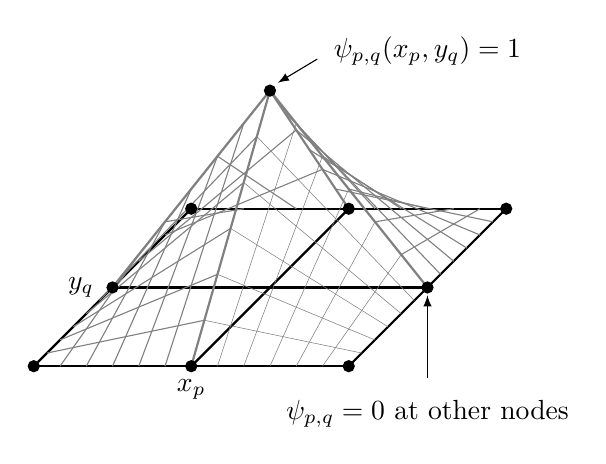
\begin{tikzpicture}[scale=0.5]

  % strong grid around elements
  \draw[thick] (0,0) -- (8,0);
  \draw[thick] (2,2) -- (10,2);
  \draw[thick] (4,4) -- (12,4);
  \draw[thick] (0,0) -- (4,4);
  \draw[thick] (4,0) -- (8,4);
  \draw[thick] (8,0) -- (12,4);

  \def\ytop{7};

  % tent lines
  \draw[gray,thick] (6,\ytop) -- (4,0);
  \draw[gray,thick] (6,\ytop) -- (2,2);
  \draw[gray,thick] (6,\ytop) -- (10,2);
  \draw[gray,thick] (6,\ytop) -- (8,4);

  \def\dx{(10.0-6.0)/6};
  \def\dy{(2.0-\ytop)/6};
  \foreach \jj in {1,...,5}
  {
       \draw[gray,very thin] ({6+\jj*\dx},{\ytop+\jj*\dy}) -- ({4+(4/6)*\jj},0.0);
  }

  \def\dx{(4.0-6.0)/6};
  \def\dy{(0.0-\ytop)/6};
  \foreach \jj in {1,...,5}
  {
       \draw[gray,very thin] ({6+\jj*\dx},{\ytop+\jj*\dy}) -- ({10-(2/6)*\jj},{2-(2/6)*\jj});
  }

  \def\dx{(2.0-6.0)/6};
  \def\dy{(2.0-\ytop)/6};
  \foreach \jj in {1,...,5}
  {
       \draw[gray,thin] ({6+\jj*\dx},{\ytop+\jj*\dy}) -- ({4-(4/6)*\jj},0.0);
  }

  \def\dx{(4.0-6.0)/6};
  \def\dy{(0.0-\ytop)/6};
  \foreach \jj in {1,...,5}
  {
       \draw[gray,thin] ({6+\jj*\dx},{\ytop+\jj*\dy}) -- ({2-(2/6)*\jj},{2-(2/6)*\jj});
  }

  \def\dx{(10.0-6.0)/6};
  \def\dy{(2.0-\ytop)/6};
  \foreach \jj in {1,...,5}
  {
       \draw[gray,thin] ({6+\jj*\dx},{\ytop+\jj*\dy}) -- ({8+(4/6)*\jj},4.0);
  }

  \def\dx{(8.0-6.0)/6};
  \def\dy{(4.0-\ytop)/6};
  \foreach \jj in {1,...,5}
  {
       \draw[gray,thin] ({6+\jj*\dx},{\ytop+\jj*\dy}) -- ({10+(2/6)*\jj},{2+(2/6)*\jj});
  }

  \def\dx{(2.0-6.0)/3};
  \def\dy{(2.0-\ytop)/3};
  \foreach \jj in {1,...,2}  % reduce clutter
  {
       \draw[gray,thin] ({6+\jj*\dx},{\ytop+\jj*\dy}) -- ({8-(4/3)*\jj},4.0);
  }

  \def\dx{(8.0-6.0)/3};
  \def\dy{(4.0-\ytop)/3};
  \foreach \jj in {1,...,2}
  {
       \draw[gray,thin] ({6+\jj*\dx},{\ytop+\jj*\dy}) -- ({2+(2/3)*\jj},{2+(2/3)*\jj});
  }

  % nodes in base plane
  \filldraw (0,0) circle (4pt);
  \filldraw (4,0) circle (4pt);
  \filldraw (8,0) circle (4pt);
  \filldraw (2,2) circle (4pt);
  %\filldraw (6,2) circle (4pt);   % (x_j,y_k) is at (6,2)
  \filldraw (10,2) circle (4pt);
  \filldraw (4,4) circle (4pt);
  \filldraw (8,4) circle (4pt);
  \filldraw (12,4) circle (4pt);

  % node at tent top
  \filldraw (6,\ytop) circle (4pt);

  % annotate
  \draw (10,\ytop+1.0) node {$\psi_{p,q}(x_p,y_q)=1$};
  \draw[-latex] (7.2,\ytop+0.8) -- (6.2,\ytop+0.2);
  \draw (10,-1.2) node {$\psi_{p,q}=0$ at other nodes};
  \draw[-latex] (10,-0.3) -- (10,1.8);

  % label center point
  \draw (4,-0.6) node {$x_p$};
  \draw (1.2,2) node {$y_q$};

\end{tikzpicture}

\caption{FIXME}
\label{fig:q1hat}
\end{marginfigure}

FIXME code uses \texttt{SNESSetObjective()} only, though also \texttt{SNESSetFunction()}; no hand-made Jacobian at all

FIXME try NCG


\section{Exercises}

\renewcommand{\labelenumi}{\arabic{chapter}.\arabic{enumi}\quad}
\renewcommand{\labelenumii}{(\alph{enumii})}
\begin{enumerate}
\item One needs to \emph{see} quadratic convergence to believe it.  Observe that for $x_k$ in both parts (b) and (c), the \emph{number of correct digits in $x_k$ doubles at each iteration}.
    \begin{enumerate}
    \item The sequence $x_k = 1-2^{-n}$ converges quickly to $x^*=1$, but not quadratically.  Find $k$ so that $|e_k| < 10^{-16}$.
    \item The sequence $x_k = 1-2^{-2^n}$ converges quadratically to $x^*=1$.  Find $k$ so that $|e_k| < 10^{-16}$.  Find the smallest $K$ so that $|e_{k+1}| \le K |e_k|^2$ for all $k$.
    \item Let $F(x) = \cos(x-1) - \exp(1-x)$ and $x_0=0.5$.  Using any quick-and-dirty numerical tool,\sidenote{Extra credit for doing it in \PETSc.} compute Newton iterates $x_k$ for $k=1,\dots,6$.  Estimate $K$ so that $|e_{k+1}| \le K |e_k|^2$ for large $k$.
    \end{enumerate}

\item Make a tiny modification to \texttt{expcircleJAC.c} to set the components of the initial vector to $20$, i.e.~$\bx_0 = [20\,\, 20]^\top$.  Rerun it only with option \texttt{-snes\_monitor} and note the manner in which it does not converge to a solution of $\bF(\bx)=0$ for \eqref{eq:nl:expcircleF}.  Why does the \pSNES stop?  Add one runtime option so that it does converge to a solution.  Is the convergence quadratic?

\item This example shows a famous case where the no-linesearch Newton iteration either diverges or enters a limit cycle according to the initial iterate $x_0$.  Linesearch fixes this.
    \begin{enumerate}
    \item By simple modifications of \texttt{expcircle.c}, write a code \texttt{e3atan.c} which solves the (one-dimensional) nonlinear equation $F(x)=\arctan(x)=0$ using initial iterate $x_0=2.0$.  Use \texttt{atan()}.  By running it \texttt{./e3atan -snes\_fd -snes\_linesearch\_type basic}, show that the Newton iteration without a linesearch diverges, while using the default choice \texttt{-snes\_linesearch\_type bt} gives convergence.
    \item Continuing with $F(x)=\arctan x$, require the Newton iteration \eqref{eq:nl:newtoneq}, \eqref{eq:nl:newtonupdate} to enter a limit cycle, i.e.~so that $x_{k+1} = - x_k$ for all $k$.  Thereby approximate the positive value $x_0$ so that the Newton iteration makes no progress, and yet remains bounded, for all $k$.\sidenote{One may solve this problem with Newton's method.}  Draw a (well-known) sketch of the situation.  Then, by modifying $x_0$ in \texttt{e3atan.c} and again using linesearch type \texttt{basic}, confirm that one can make the Newton iteration ``stick'' in this (actually unstable) limit cycle for quite a while.  Then confirm that linesearch types \texttt{bt,l2,cp} all get unstuck immediately.
% to solve:  - x = x - arctan(x) (1+x^2)
% octave:
%   G = @(x) 2*x - atan(x) * (1+x^2);
%   J = @(x) 1 - atan(x) * (2*x);
%   x = 1.4;
%   format long g
%   for j = 1:4, x = x - G(x) / J(x), end
% get:
%  x = 1.39174520027073

    \end{enumerate}

\end{enumerate}